\documentclass[menu.tex]{subfiles}
\graphicspath{ {images/} }
\begin{document}            
    
    \begin{tabular} {p{3.5cm} p{4cm} p{9cm}}        
    \multicolumn{3} { c }{\begin{LARGE}Menú Semanal 2\end{LARGE}}\\
    \hline
    
    %---LUNES---%
\pbox{20cm}
{
\rule{0pt}{3ex}\begin{large}\textbf{Lunes}\end{large}\\ 
\rule{0pt}{2ex}Atún con \\cebollines \\
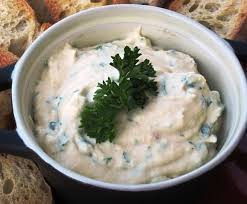
\includegraphics[scale=0.4]{atun-cebollines} 
} & 
\vspace{-2cm}
\begin{compactitem} 
\begin{footnotesize}
\item \nicefrac{1}{2} lata de atún
\item 1 manojo de cebollin picado
\item 1 manojo de perejil picado
\item Mayonesa light
\item Lechuga
\end{footnotesize}
\end{compactitem}&
\vspace{-2cm}
Mezcla media lata de atún al agua con los cebollines picados a gusto (recomendable una cantidad generosa). Agregar perejil picado a gusto (para un sabor potente se recomienda una buena cantidad) y mayonesa light. Mezclar todos los ingredientes, servir sobre una hoja de lechuga y acompañar con otros vegetales.\\
\hline
    
    %---MARTES---%
\pbox{20cm}
{
\rule{0pt}{3ex}\begin{large}\textbf{Martes}\end{large}\\
\rule{0pt}{2ex}Albóndigas rellenas\\
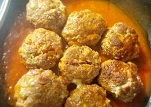
\includegraphics[scale=0.0092]{albondigas-rellenas}
}&
\vspace{-1.6cm}
\begin{compactitem} 
\begin{footnotesize}
\item Albóndigas de res o atún
\item Salvado de trigo
\item Jamón
\item Queso
\item Huevo
\end{footnotesize}
\end{compactitem}&
\vspace{-1.6cm}
Prepare las albóndigas tal como sabe hacerlas, solo que, en vez de usar pan molido, utilice salvado de trigo o de avena muy bien molidos (si la marca que compro no viene bien molida, licue el salvado en seco hasta que se parezca a la harina). Haga un hueco en la albóndiga y rellene con queso y jamón picados en forma fina, cocinarlos en aceite. Aplane la preparación sin rellenar y tendrás unas agradables hamburguesas dietéticas. Use poco huevo para no requerir mucho salvado ya que este al ser cocidos tiende a endurecerse. Puede probar la misma preparación en base a atún al agua.\\
\hline
    
    %---MIERCOLES---%
    \pbox{20cm}
    {
        \rule{0pt}{3ex}\begin{large}\textbf{Miércoles}\end{large}\\ 
        \rule{0pt}{2ex}Ensalada de pollo\\
        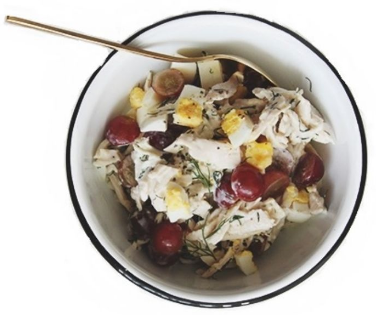
\includegraphics[scale=0.4]{ensalada-de-pollo} 
    } & 
    \vspace{-2cm}            
    \begin{compactitem} 
        \begin{scriptsize}
            \item 2 tazas de pollo troceado
            \item 1 taza de uvas rojas (u otro tipo) cortadas a la mitad
            \item 2 huevos cocidos y troceados
            \item Mayonesa (mejor casera)
            \item Un poquito de eneldo fresco
            \item 1 diente de ajo picado
            \item Sal
            \item Pimienta
        \end{scriptsize}
    \end{compactitem}&
    \vspace{-2cm}        
    Fríe el pollo en una sartén con aceite de oliva. Reserva.
    En un bol, coloca el pollo, añade el resto de ingredientes y mezcla bien.
    Nota: puedes conservarlo en el frigorífico tapado con film transparente.\\
    \hline
    %---JUEVES---%
    \pbox{20cm}
    {
        \rule{0pt}{3ex}\begin{large}\textbf{Jueves}\end{large}\\ 
        \rule{0pt}{2ex}Ensalada caprese con pollo\\
        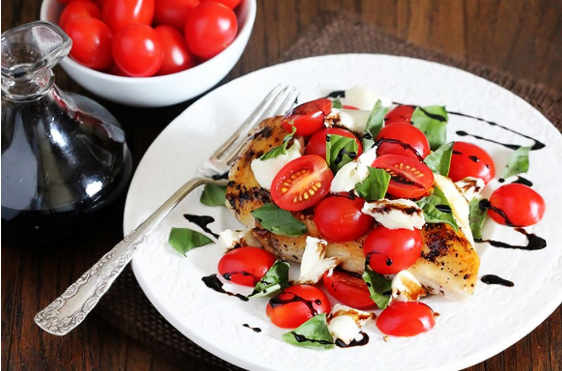
\includegraphics[scale=0.26]{ensalada-caprese-con-pollo} 
    } & 
    \vspace{-1.6cm}
              
    \begin{compactitem} 
        \begin{scriptsize}
            \item Bolitas de mozzarella marinadas
            \item Pechuga de pollo
            \item Tomates cherry
            \item Pimienta molida
            \item Sal
            \item Aceite de oliva
        \end{scriptsize}
    \end{compactitem} &
    \vspace{-1.6cm}     
    Saca las bolitas de mozzarella de su marinada y vierte la mitad de la marinada en un bol.
    Coloca el pollo en el bol con marinada, sazona con sal y pimienta y déjalo reposar durante 1 hora a temperatura ambiente.
    Corta las bolitas de mozzarella, ponlas en un bol aparte y añade la otra mitad de marinada. Reserva.
    Añade los tomates cherry al bol de la mozzarella y sazona con sal y pimienta. Reserva.
    Cocina la pechuga de pollo a la plancha dejando que se tueste un poco y córtala en pequeños cubos.
    Añade los trocitos de pollo al bol con la mozzarella y los tomates, mezcla y sirve.\\
    \hline
    
    %---VIERNES---%
    \pbox{20cm}
    {
        \rule{0pt}{3ex}\begin{large}\textbf{Viernes}\end{large}\\ 
        \rule{0pt}{2ex}Ensalada de brócoli\\ y manzana\\
        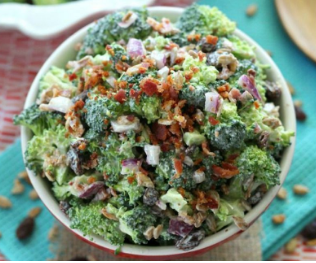
\includegraphics[scale=0.4]{ensalada-brocoli-manzana} 
    } & 
    \vspace{-2cm}
    \begin{compactitem} 
        \begin{footnotesize}
            \item 2 tazas de de brócoli
            \item 1 manzana pelada en cubitos
            \item Nueces tostadas y troceadas
            \item Fruta deshidratada
            \item 3 lonchas de tocino
            \item 1 cucharilla de miel
            \item Vinagre
            \item \nicefrac{1}{2} taza de mayonesa
            \item Sal
            \item Pimienta
            \item Aceite de oliva
        \end{footnotesize}
    \end{compactitem}&
    \vspace{-2cm}
    Trocea el tocino y cocínalo a la plancha con unas gotas de aceite de oliva. Reserva.
    Introduce el brócoli en agua hirviendo durante un minuto y enfríalo bajo el grifo. Escurre y reserva.
    Coloca en un bol el brócoli, la manzana, las nueces, la fruta deshidratada y el tocino. Reserva.
    En otro bol, mezcla la miel, el vinagre y la mayonesa hasta conseguir un aderezo de consistencia suave.
    Sazona el aderezo con sal y pimienta.
    Añade el aderezo al bol con el brócoli y el resto de ingredientes y mezcla bien.
    Nota: puedes ajustar las cantidades de ingredientes usados para el aderezo según tus gustos. \\
    \hline
    
    %---SABADO---%
    \pbox{20cm}
    {
        \rule{0pt}{3ex}\begin{large}\textbf{Sabado}\end{large}\\ 
        \rule{0pt}{2ex}Ensalada de tomate,\\ tocino y aguacate \\
        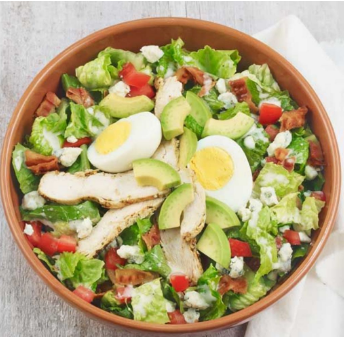
\includegraphics[scale=0.4]{ensalada-bacon-palta} 
    } & 
    \vspace{-2.4cm}
    \begin{compactitem} 
        \begin{footnotesize}
            \item 1 aguacate maduro
            \item 1 tomate
            \item 2 huevos cocidos
            \item 3 lonchas de tocino
            \item Sal
            \item Pimienta
            \item Zumo de limón
            \item Aceite de oliva
        \end{footnotesize}
    \end{compactitem}&
    \vspace{-2.4cm}
    Cocina el tocino a la plancha con unas gotas de aceite de oliva y córtalo en trozos muy pequeños. Reserva.
    Trocea el aguacate, los huevos y el tomate. Reserva.
    Exprime uno o dos gajos de limón para obtener el zumo.
    Coloca el aguacate, los huevos, el tomate y el tocino en un bol.
    Sazona con sal y pimienta y añade el zumo de limón.
    Mézclalo todo bien y sirve.\\
    \hline

    \newpage        
    \end{tabular}
\end{document}
